\subsection{Submit Problem}

\begin{frame}
\begin{figure}[htbp]
\begin{center}
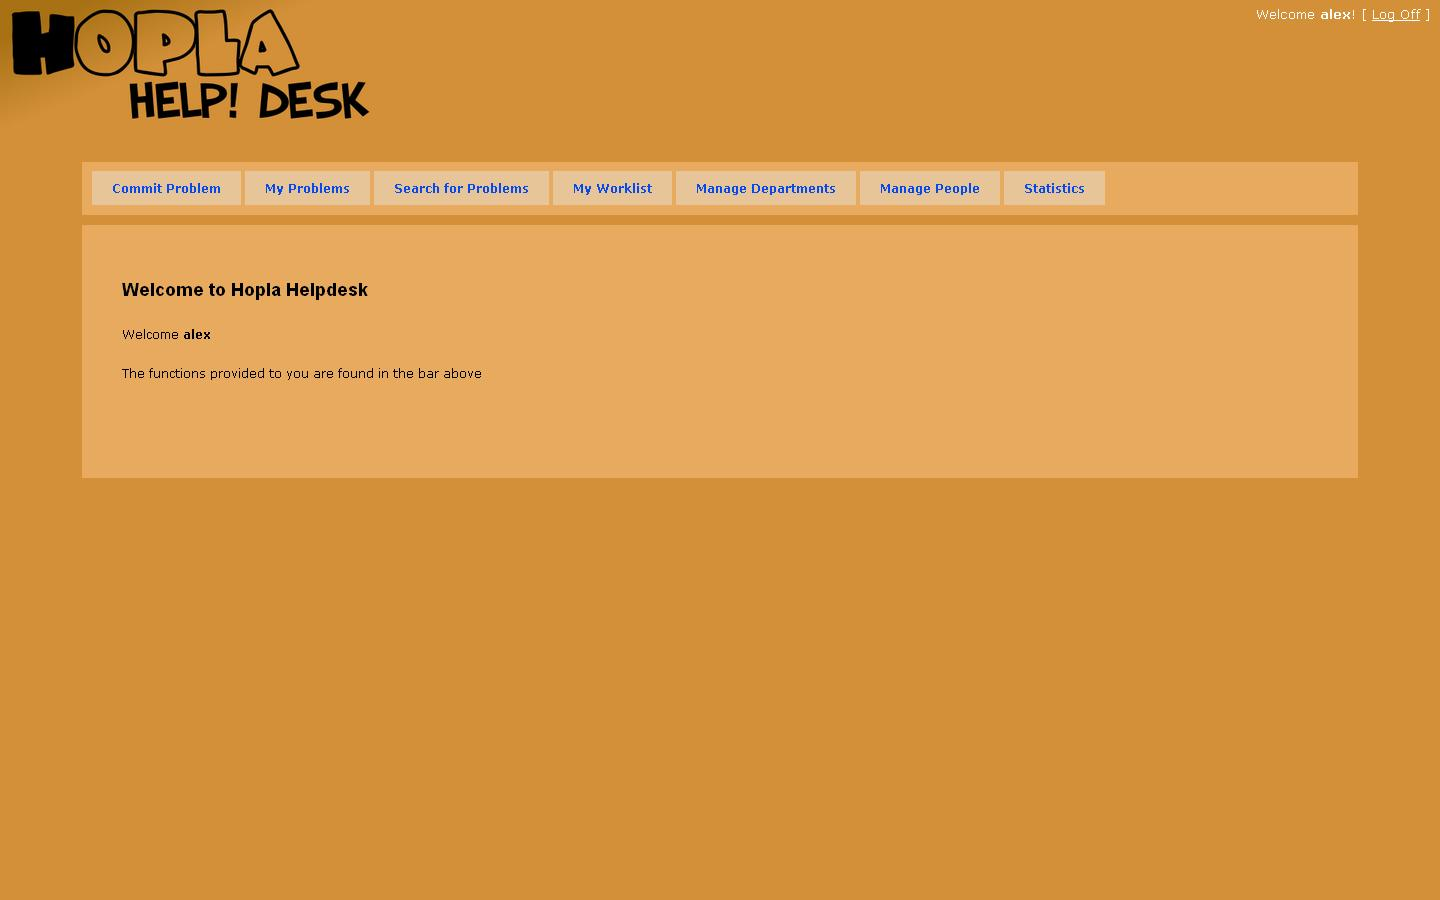
\includegraphics[clip=true,trim=0cm 9cm 16cm 0cm,width=\textwidth]{input/search/home.JPG}
%\caption{default}
%\label{default}
\end{center}
\end{figure}

\end{frame}

\begin{frame}

\begin{figure}[htbp]
\begin{center}
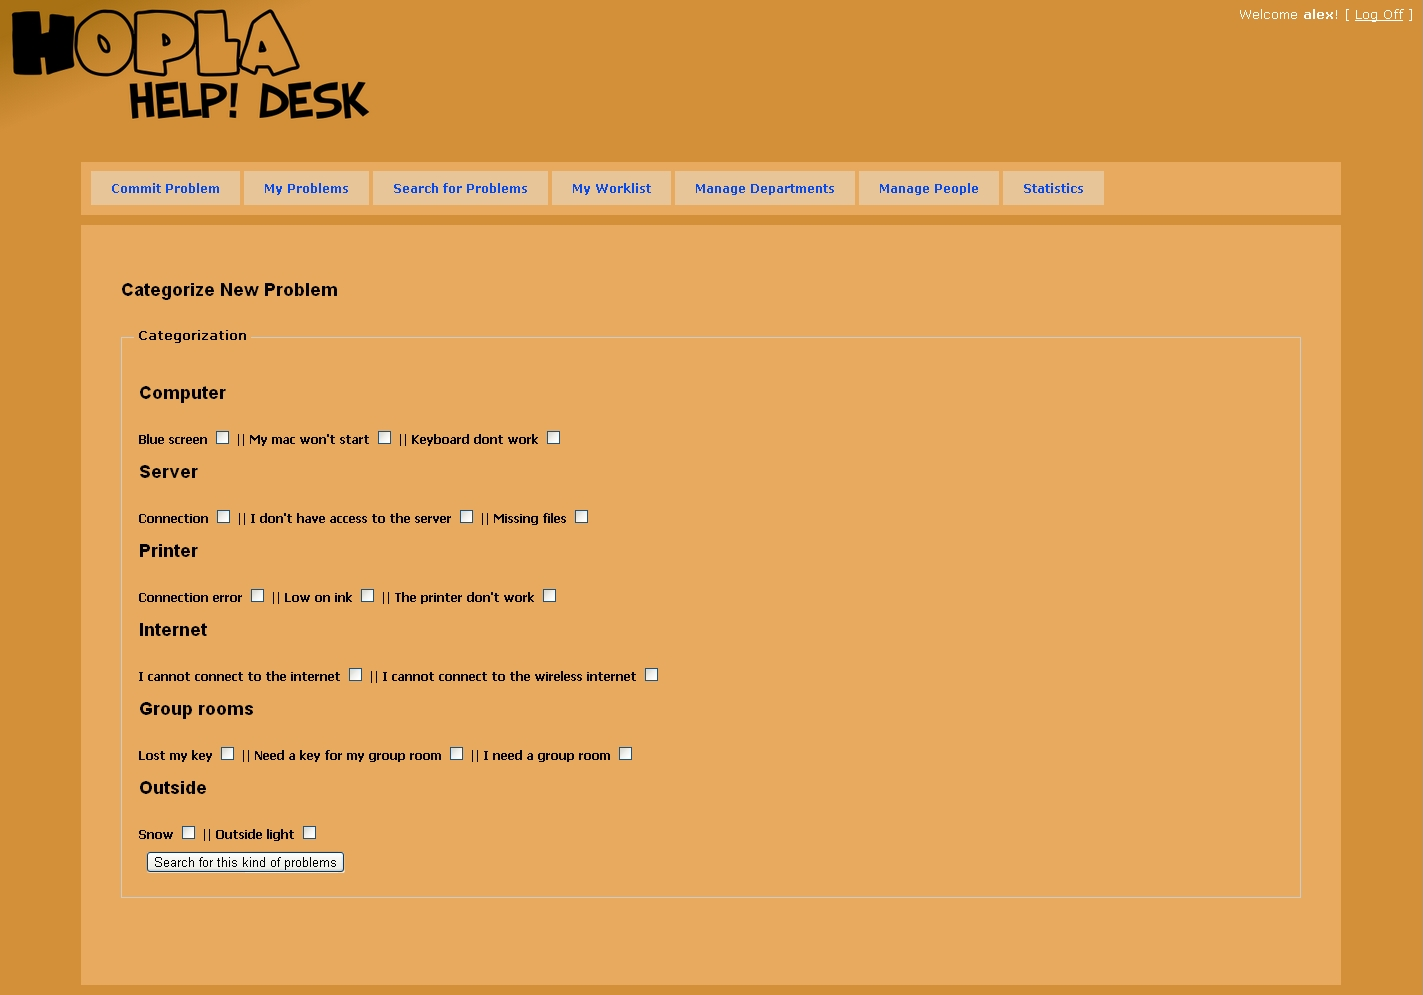
\includegraphics[clip=true,trim=0cm 2cm 16cm 0cm,width=\textwidth]{input/search/commit.png}
%\caption{default}
%\label{default}
\end{center}
\end{figure}

\end{frame}

\begin{frame}

\begin{figure}[htbp]
\begin{center}
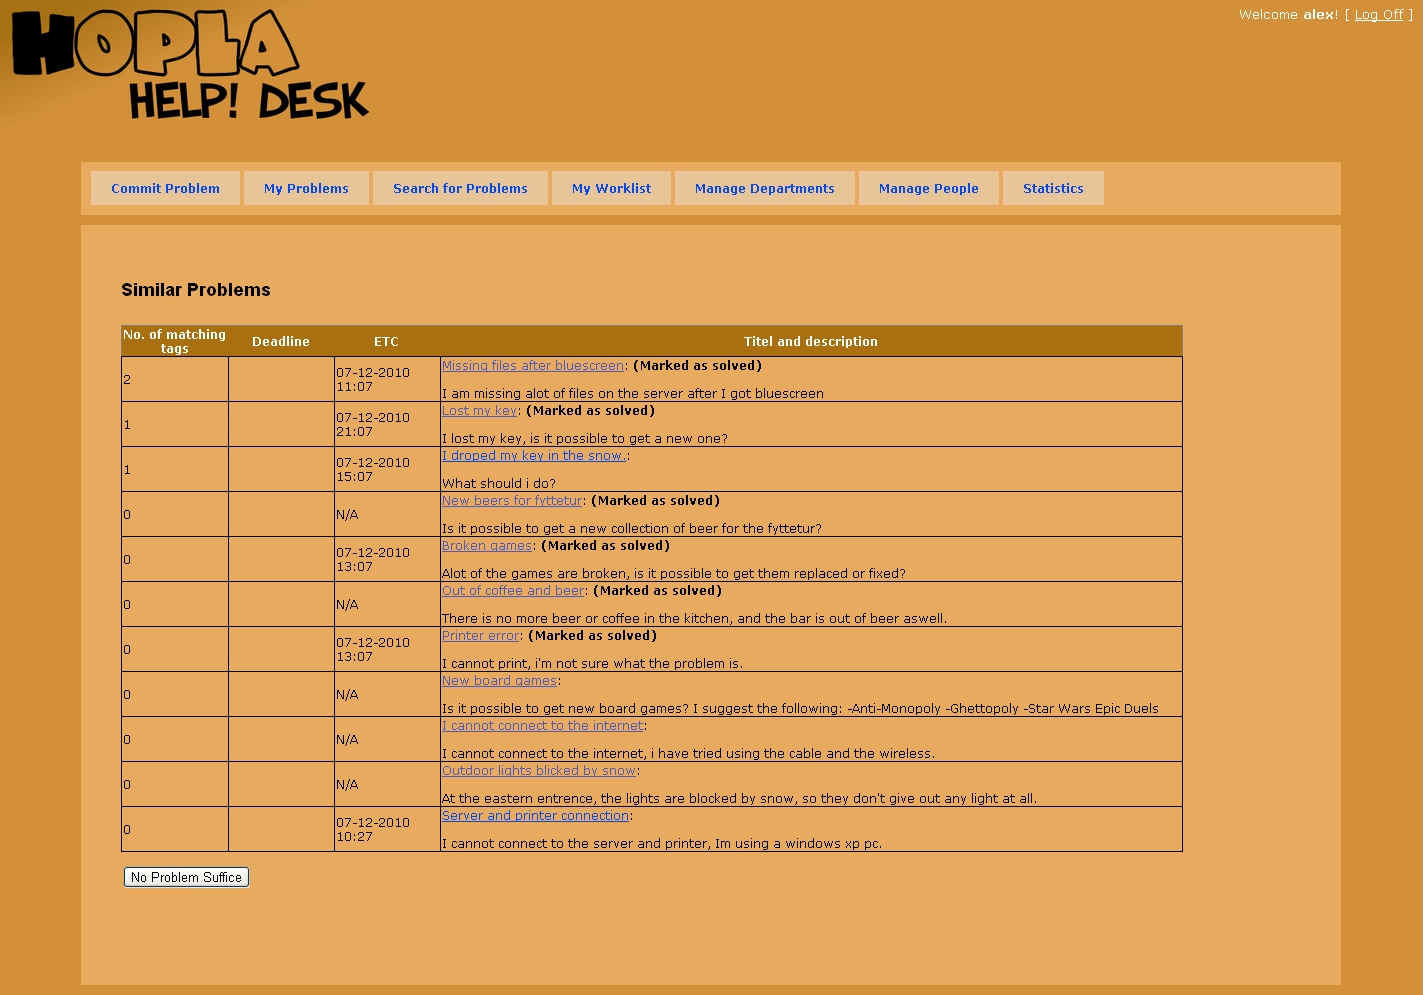
\includegraphics[clip=true,trim=2cm 2cm 16cm 9cm,width=\textwidth]{input/search/similarProblems.png}
%\caption{default}
%\label{default}
\end{center}
\end{figure}

\end{frame}

\begin{frame}

\begin{figure}[htbp]
\begin{center}
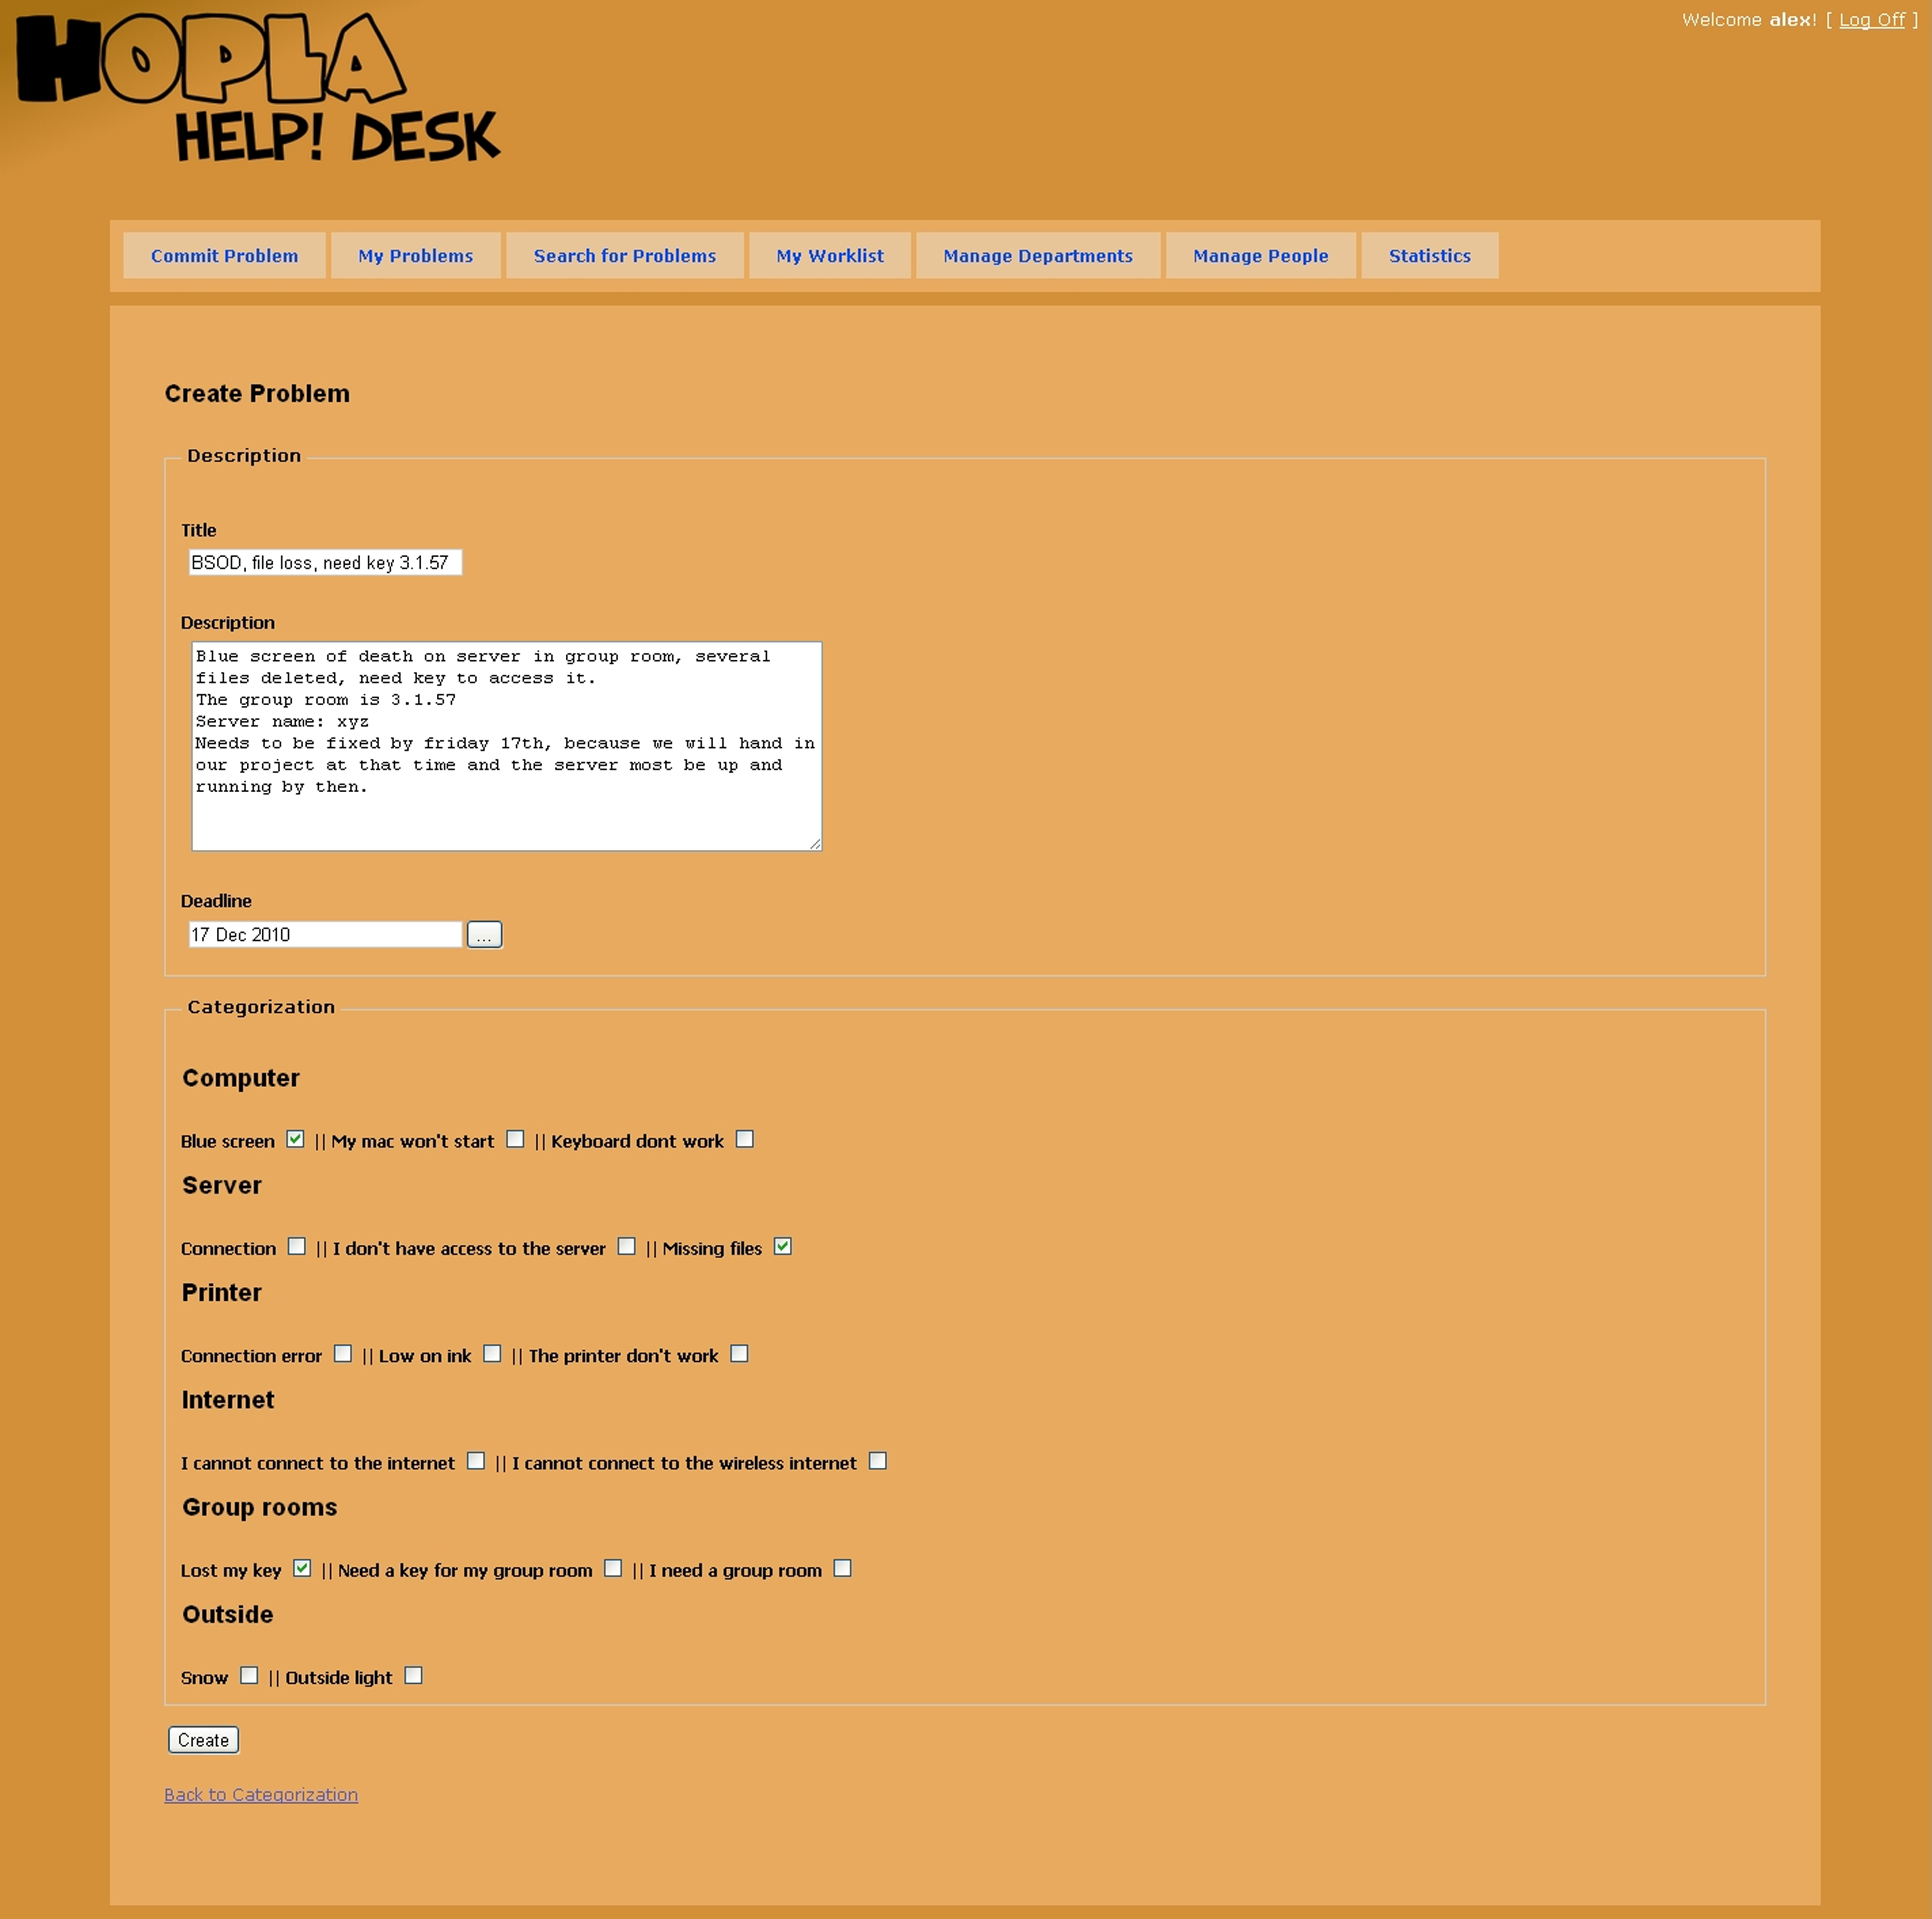
\includegraphics[clip=true,trim=3.5cm 0cm 9cm 9.5cm,width=\textwidth]{input/search/newProblem2.png}
%\caption{default}
%\label{default}
\end{center}
\end{figure}

\end{frame}
% The interresting here is  the search, we try search a set of problems

\newcommand{\tagone}{Computer}
\newcommand{\tagtwo}{BSOD}
\subsubsection{Search}
\begin{frame}{The Search}
\begin{itemize}
	\item Tags to search: \tagone{} + \tagtwo{}
	\only<2->{\item Minimum number of problems to find: 3}
 	\only<3>{ \item Problems to search in: }
	\only<4>{ \item Results: }
	\only<3-4>{\begin{itemize}}
		\only<3>{\item A - \tagone{} }
		\only<3>{\item B - \tagtwo{} }
		\only<3>{\item C -\tagone{} + \tagtwo{} }
		\only<3>{\item D - \tagone{} + \tagtwo{} + Internet  }
		\only<3>{\item E - \tagone{} + Internet }
		\only<3>{\item F - Internet }
	
		\only<4>{\item C - \tagone{} + \tagtwo{} }
		\only<4>{\item D - \tagone{} + \tagtwo{} + Internet}
		\only<4>{\item B - \tagtwo{}}
		\only<4>{\item A - \tagone{}}
		\only<4>{\item E - \tagone{} + Internet}
	\only<3-4>{\end{itemize}}
\end{itemize}

\end{frame}


